\chapter{Future Work}

\begin{figure}[ht]
\centering
		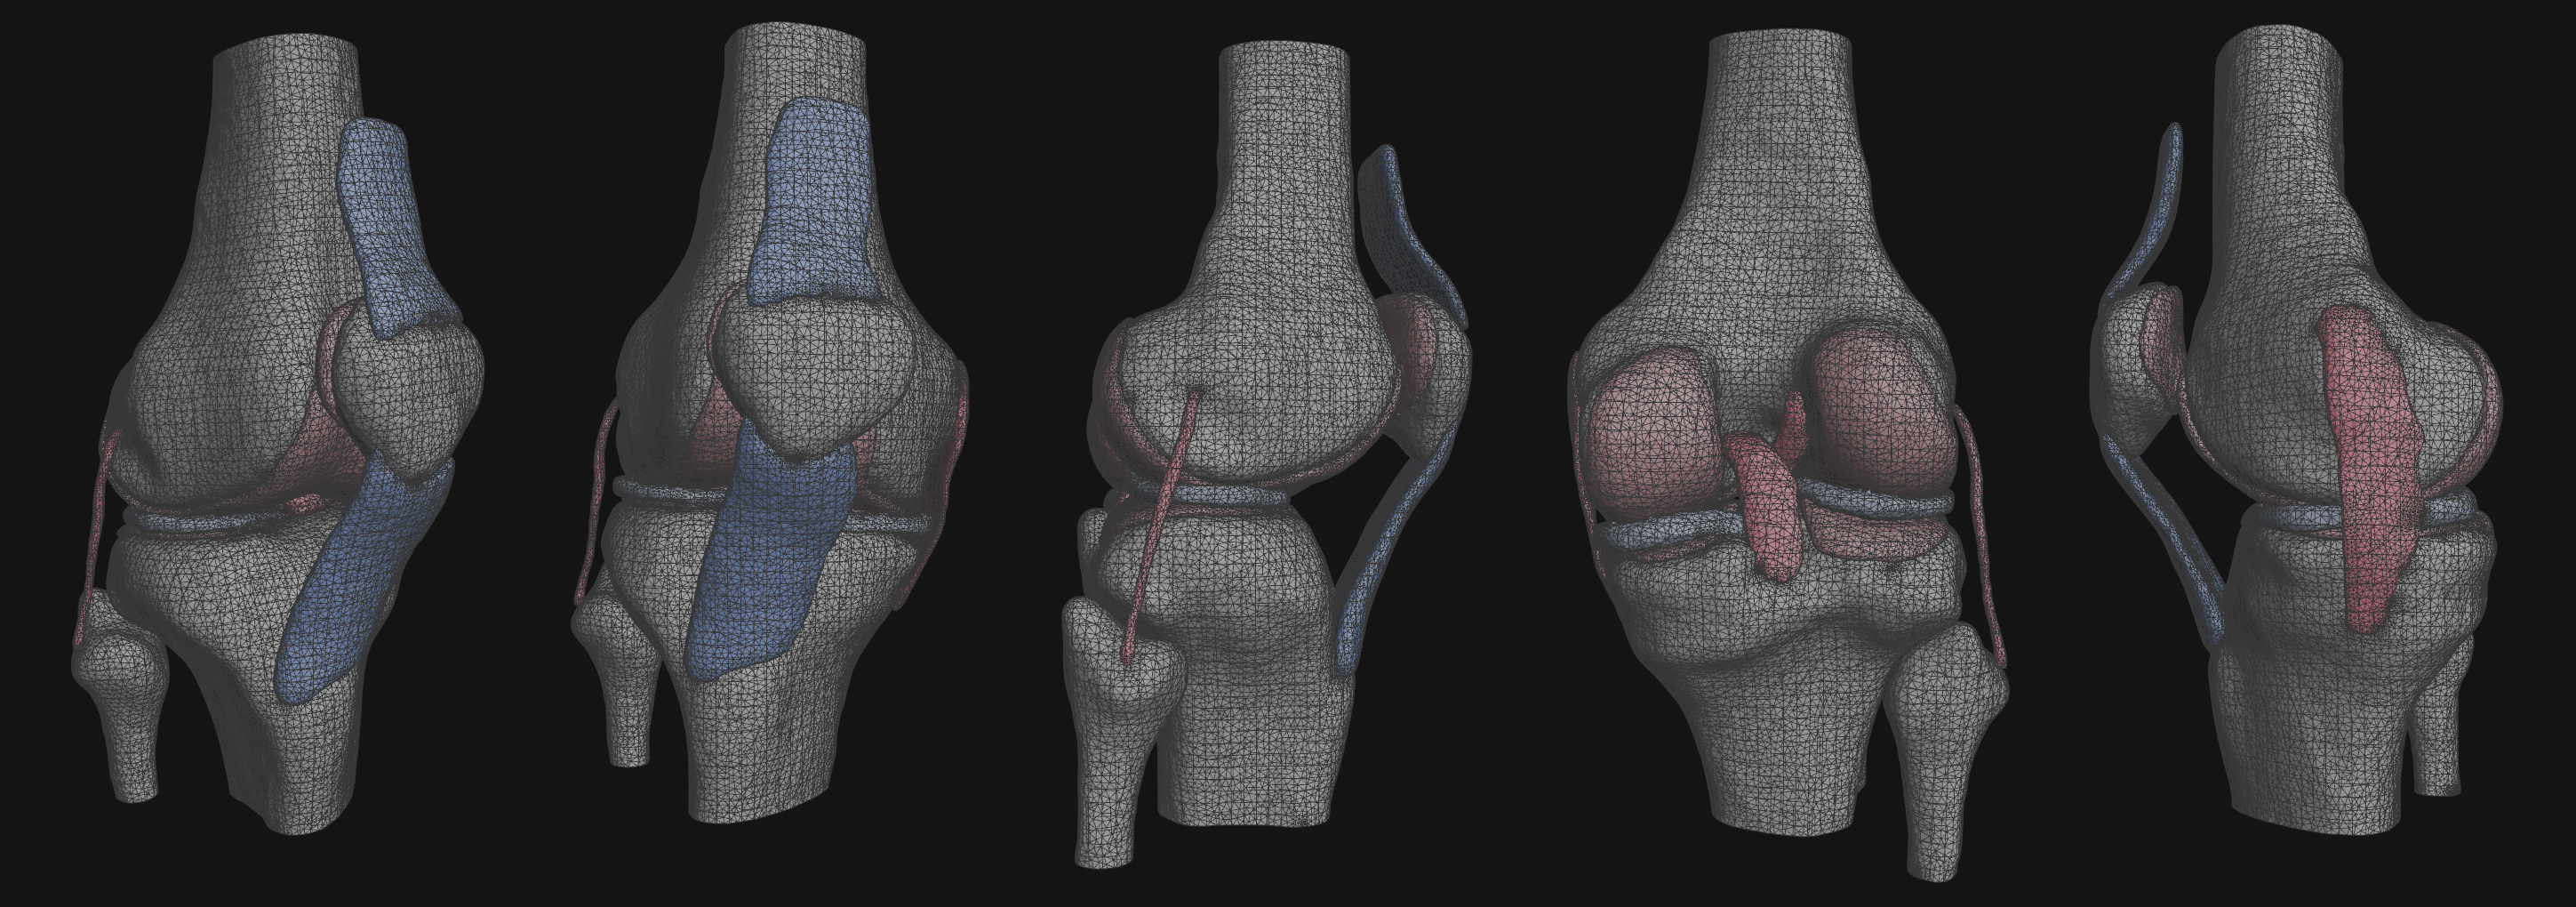
\includegraphics[width=1.0\textwidth]{media/7-polyknee/fullmesh.png}
%
\caption{Polyhedral mesh of human knee from input surfaces generated from OpenKnee image masks}
\label{fig:polyknee}
\end{figure}

\begin{figure}[ht]
\centering
		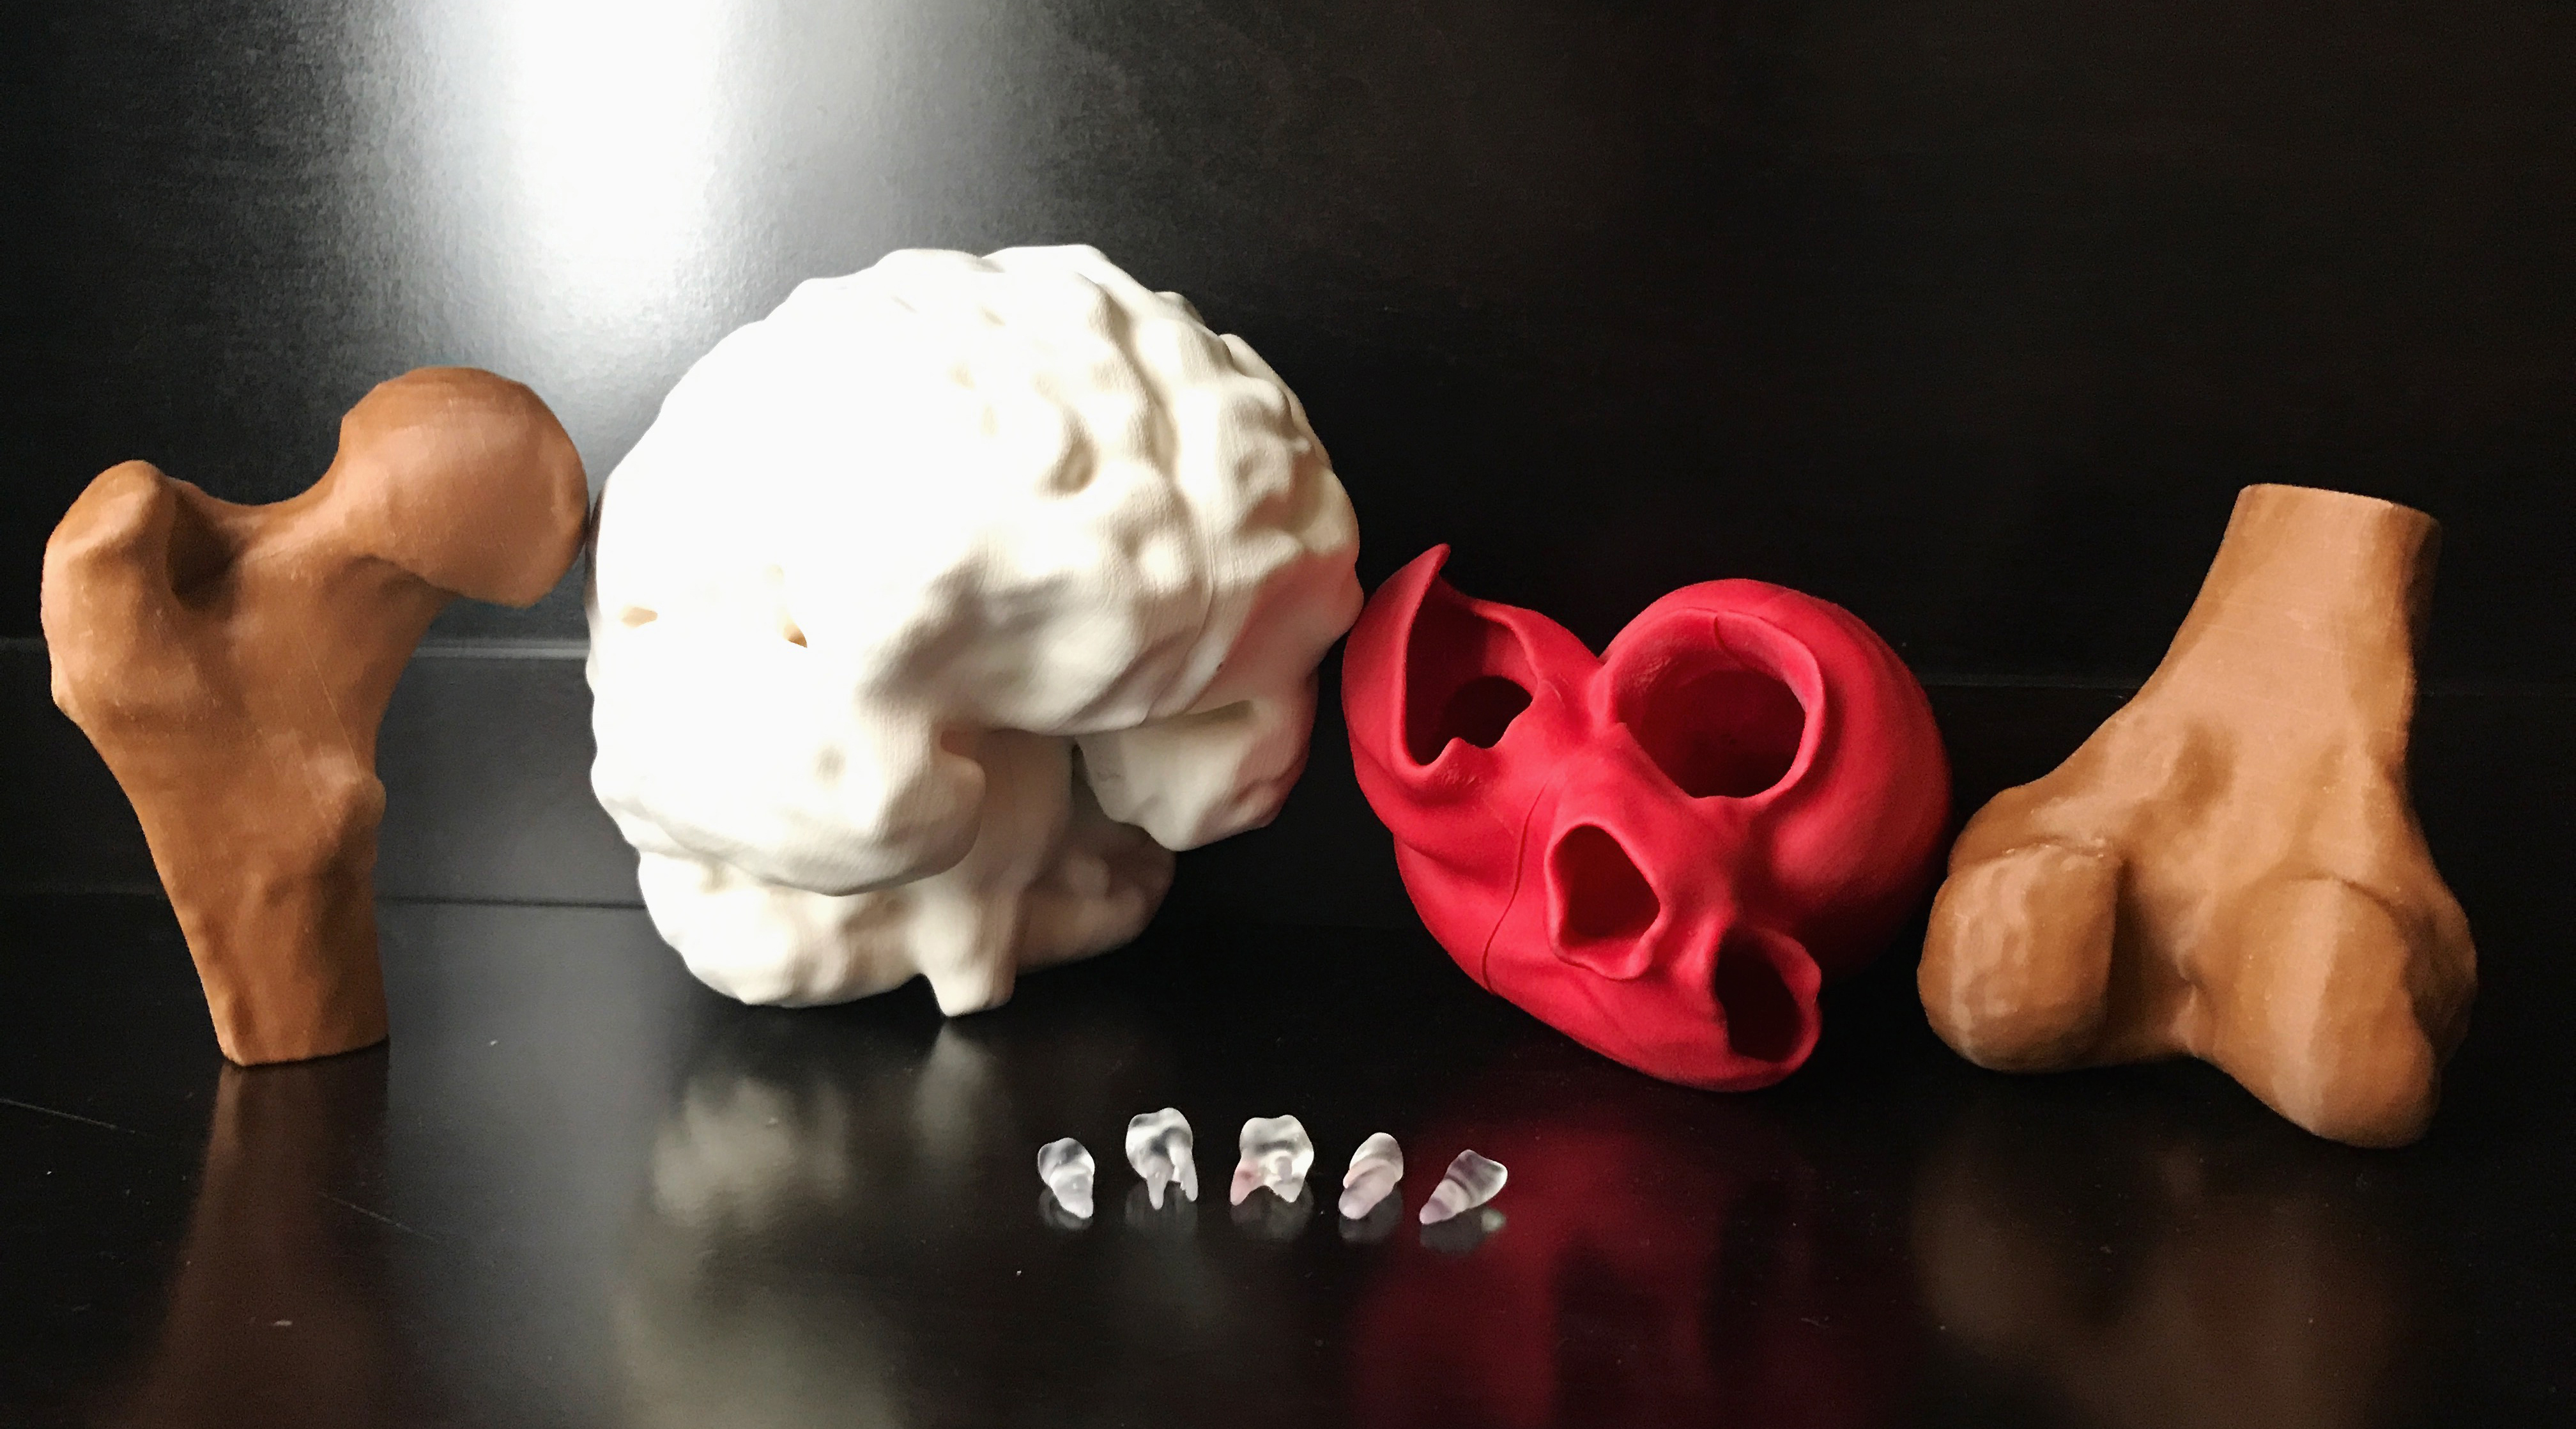
\includegraphics[width=1.0\textwidth]{media/6-3dprint/3dprint.jpg}
%
\caption{Suite of 3D-printed organs using surface meshes generated from novel image-based meshing tools}
\label{fig:3dprint}
\end{figure}

%%%%%%%%%%%%%%%%%%%%%%
%%%%%%%%%%%%%%%%%%%%%%
\section{Short Term}
\label{Short Term}

\subsection[A Polyhedral Finite Element Demonstration in Cardiac \newline Mechanics]{\texorpdfstring{A Polyhedral Finite Element Demonstration in Cardiac \newline Mechanics}{A Polyhedral Finite Element Demonstration in Cardiac \newline Mechanics}}
\label{A Polyhedral Finite Element Demonstration in Cardiac Mechanics}

\subsection[A Machine Learning System to Guide Clinical Procedures in \newline Real-Time]{\texorpdfstring{A Machine Learning System to Guide Clinical \newline Procedures in Real-Time}{A Machine Learning System to Guide Clinical \newline Procedures in Real-Time}}
\label{A Machine Learning System to Guide Clinical Procedures in Real-Time}

\subsection{Improvements to Image-Based Meshing Code}
\label{Improvements to Image-Based Meshing Code}
direct surface generation from image \\
multiple materials \\
tolerance-aware voronoi partitioning \\
use of soft segmentations/handling of partial volume effect  \\
numerical validation of segmentation and of surface

\subsection{Improvements to Cardiac Mechanics Code}
\label{Improvements to Cardiac Mechanics Code}
run PEM version in Celeris \\
BCs, etc.

%%%%%%%%%%%%%%%%%%%%%%
%%%%%%%%%%%%%%%%%%%%%%\\
\section{Long Term}
\label{Long Term}

\subsection[Applications in Rapid Prototyping and Additive Manufacturing]{\texorpdfstring{Applications in Rapid Prototyping and Additive \newline Manufacturing}{Applications in Rapid Prototyping and Additive \newline Manufacturing}}
\label{Applications in Rapid Prototyping and Additive Manufacturing}

\subsection{\textit{In Silico} Modeling}
\label{In Silico Modeling}
Simulation of Clinical trials


